\documentclass[oneside,13pt,a4paper]{article}

% Chargement d'extensions
\usepackage[utf8]{inputenc}
\usepackage[french]{babel}
\usepackage{graphicx}
\usepackage[top=3cm, bottom=3cm, left=2.5cm, right=2.5cm]{geometry}
\usepackage{amsmath}
\usepackage{amssymb}

% Liens et autres
\usepackage{hyperref}
\hypersetup{
    colorlinks=true,
    linkcolor=black,
	urlcolor=blue,
	pdftitle={Air France},
	bookmarks=true,
}

% Bout de code
\usepackage{listings}
\usepackage{color}

% Commande pour notation 'NB :' (nota bene)
\newcommand\nb[1][0.3]{N\kern-#1emB : }

% csquotes va utiliser la langue définie dans babel
\usepackage[babel=true]{csquotes}
\usepackage{array,multirow,makecell}
\usepackage{tabularx}

% pour afficher Schéma au lieu de figure dans les legende des images
\addto\captionsfrench{\def\figurename{Schéma}}

% Informations le titre, le(s) auteur(s), la date
\title{}
\author{
    Belkassim BOUZIDI \and
    Chakib ELHOUITI \and
    Massili KEZZOUL \and
   
}
\date{\today}


\begin{document}
%\maketitle
\begin{titlepage}
  \centering
  {\scshape\LARGE Universite de Montpellier\par}
  {\scshape\Large\par}
  \vspace{1.5cm}
  {\huge\bfseries Rendu mini projet Entrepôt de données\\Air France\par}
  \vspace{2cm}
  {\Large\itshape
    Belkassim BOUZIDI \\
    Chakib ELHOUITI \\
    Massili KEZZOUL \\

    \par}





  \vspace{2cm}

  \begin{figure}[h]
    \begin{minipage}[c]{.46\linewidth}
      \centering
      
\includegraphics[width=1\textwidth]{img/univ-montpellier.png}
    \end{minipage}
    \hfill%
    \begin{minipage}[c]{.46\linewidth}
      \centering
      
\includegraphics[width=1\textwidth]{img/fds.png}
    \end{minipage}
  \end{figure}

  \par\vspace{1cm}

  \vfill

  % Bottom of the page
  {\large \today\par}
\end{titlepage}




% ------------------------------------- %
% Introduction
% ------------------------------------- %

\parskip=5pt

\vspace{\stretch{1}}

\parskip=0pt


% Espacement entre les paragraphes
\parskip=5pt
% ------------------------------------- %
% Organisation
% ------------------------------------- %
\section{Présentation de l'entreprise : }
Air France est la compagnie aérienne nationale française, fondée le 7 octobre 1933. Ses activités principales sont le transport de passagers, de fret ainsi que la maintenance et l'entretien des avions. Elle dessert les principaux aéroports français ainsi que de nombreux aéroports étrangers.

\section{Analyse complète d'Air France : }

\subsection{Objectifs de l'entreprise : }

Le premier objectif d'Air Fance est de développer son réseau, de développer ses possibilités de destinations tout en réduisant les coûts. Au même temps assurer une prestation de service de haute qualitée.

\subsection{Position de l'entreprise sur le marché : }
Air France est l'une des leader du transport aérien européan. Elle est longtemps rester sur une image de chic à la française en proposant pour ses clients des services haut de gammes. Mais depuis l'arrivé des vols low-cost, Air France est en baisse de revenu ce qui l'a poussé à proposer pour tous ces vols des billet au prix reduit (seconde classe).

\subsection{Quelques chiffres d'Air France : }
\begin{itemize}
  \item 104 Millions de passagers en 2019.
  \item 200 clients internationaux (maintenance).
  \item 391 destination (activité cargot).
  \item 302 avions en 2019.
  \item 308 destinations (activité passsager en 2019) dans 116 pays.
  \item L'activite passager represente 80\% du chiffre d'affaire.
  \item 6 avions cargot.
  \item 15,8 Milliard d'euro de chiffre d'affaire en 2017.
\end{itemize}

\subsection{Service proposés par l'entreprise : }
Air France proposent plusieurs types de services, notament :
\begin{itemize}
  \item Transpoirt de voyageurs (avec 80\% du CA).
  \item Transport de marchandise.
  \item Maintenance et entretien des avions.
\end{itemize}

\subsection{Formes de revenu et dépenses :}

\subsubsection{Revenu :}

\begin{itemize}
  \item Ventes de billet;
  \item Ventes de services à bords de l'avion;
  \item Transport de personnes;
  \item Transport de marchandise;
  \item Maintenance aéronautique
\end{itemize}

\subsubsection{Dépenses :}

\begin{itemize}
  \item Carburant,
  \item Le coût de l’équipage,
  \item La maintenance de l'avion,
  \item L'achat de nouveaux avions...
\end{itemize}


\subsection{Information aidant la prise de décision :}

\begin{itemize}
  \item Déterminer quel sont les liaisons les plus demander, en quel période.
  \item Pour un vol donner à quel prix peut se vendre un billet pour remplir au maximum l'avion.(les prix maximum pour remplir l'avion)
  \item Connaître la tranche d'age de clients pour de promotions.
  \item Quels sont les distination en vogue en ce moment. (si une nouvelle destination apparait)
  \item Déterminer si un vol rapporte plus ou moins qu'un autre vol.
  \item Quelle est la positon de chaque avion (Gérer au mieux la flotte d'avions disponible).
  \item la rentabilité de chaque type avion (Exemple: consommation trop forte de carburant d'un avion => le remplacer par un autre)
\end{itemize}

\section{Q2 Les actions et opérations à tracer pour récupérer ces informations. : }

\begin{itemize}
  \item Ventes des billets/vols
        \begin{itemize}
          \item la date de la vente.
          \item le lieux de depart et d'arrivé(distination en vogue).
          \item le prix de vente du billet.
          \item Nombre de place occupé dans l'avion.
          \item rentabilité du vol (revenu/dépenses)
          \item La tranche de chaque client. 
          \item La fidelité de chaque client.
          \item Nombre de billets enregistrés pour chaque client 
        \end{itemize}
\end{itemize}
\begin{itemize}
  \item Gestion des stocks d'avions
        \begin{itemize}
          \item position de chaque avion à la fin de la journée (aéroports)
          \item consommation d'un avion (carburant et divers coûts)
          \item nombre de vol effectués par un avion.
        \end{itemize}
\end{itemize}

\section{Q3 Traitement possibles : }

\begin{itemize}
  \item Ventes des billes/vols
        \begin{itemize}
          \item Analyser la demande vers une destination (le nombre de billets vendu) selon la période
          \item Analyser le ratio nombre de place occupé / capacité dans l'avion pour calculé le prix du billet
          \item Comparer le ratio revenu / dépenses pour chaque vol (rentabilité)
        \end{itemize}
\end{itemize}
\begin{itemize}
  \item Gestion des stocks d'avions
        \begin{itemize}
          \item Analyser la position de chaque avion à la fin d'une journée.
          \item Analyser le coût moyen d'un avion en carburant.
          \item Comparer les rentabilité des avions(CÀD: recettes - dépenses).
        \end{itemize}
\end{itemize}

\section{Q4 Ordonnez les actions par ordre d’importance / rentabilité potentielle : }
\begin{enumerate}
  \item Ventes des billets
  \item Organisation des avions et vols
\end{enumerate} 

\section{Q5 Identifiez les deux actions / opérations les plus importantes à analyser : }

\begin{enumerate}
  \item Ventes des billets
  \item Organisation des avions et vols
\end{enumerate}

\section{Q6 et Q7 Data-Mart}

\subsection{Data-Mart ventes des billets}

\begin{figure}[h]
  \centering
  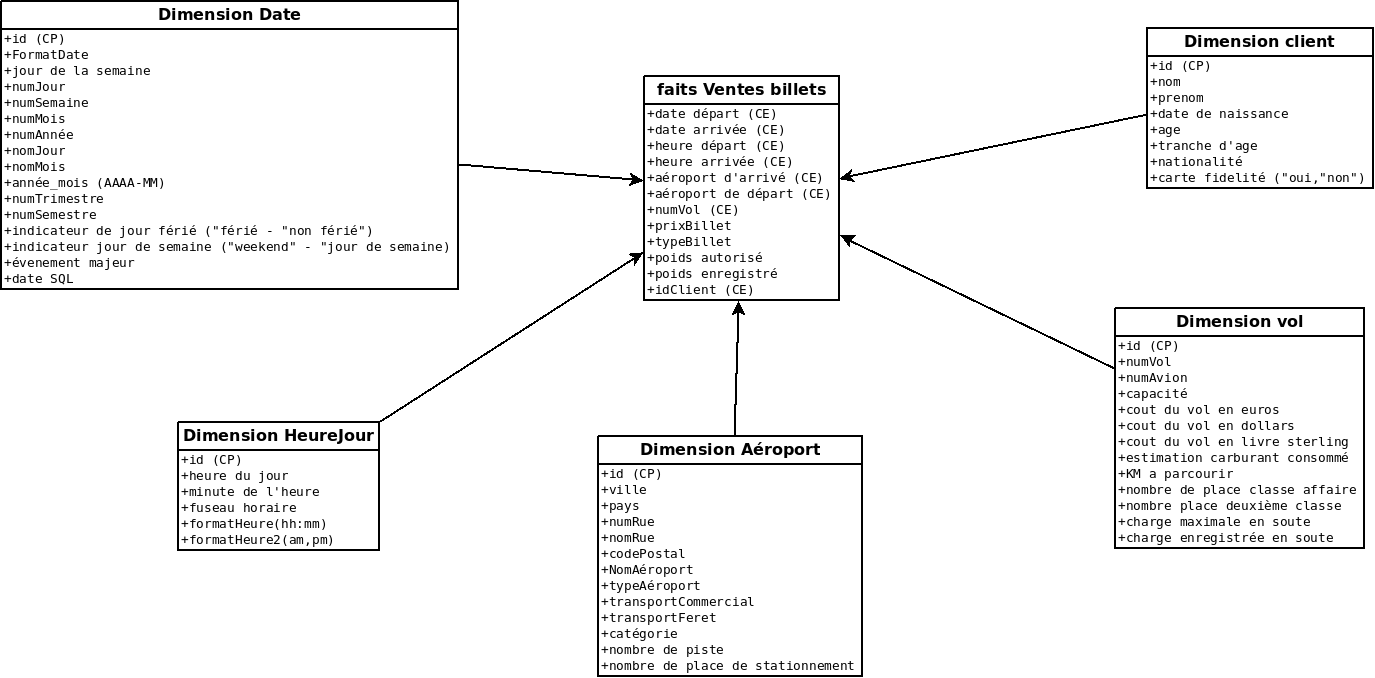
\includegraphics[width=1\textwidth]{img/VenteBillet.png}
  \caption{Data-Mart Ventes de Billets}
\end{figure}

Pour chaque billet vendu, on enregistre les mesures suivantes :
\begin{itemize}
  \item Le prix du Billet - Additive
  \item Le type du Billet (1-ére class, seconde classe ..) - Non-Additive
  \item Le poids enregistré - Additive
\end{itemize}

\begin{figure}[h]
  \centering
  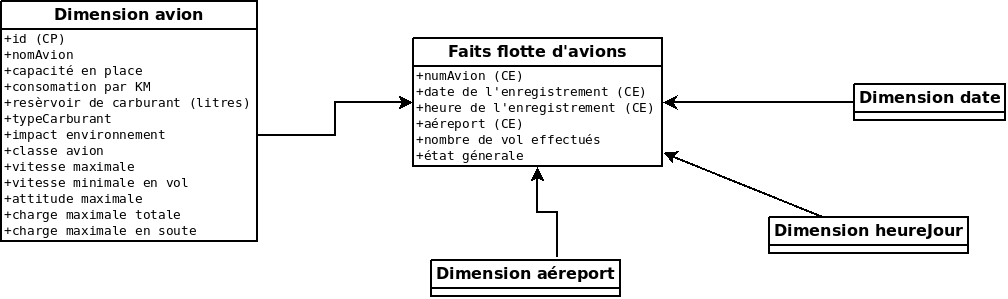
\includegraphics[width=1\textwidth]{img/flotteAvions.png}
  \caption{Data-Mart Gestion de la flotte}
\end{figure}

Une ligne de cette table des faits represente un avion à un certain moment. Les mesures sont :
\begin{itemize}
  \item Le nombre de vol effectués par l'avion - Additive
  \item Le nombre de KM parcouru par l'avion - Additive
  \item Carburant consommé - Additive
  \item recette - Additive
\end{itemize}

\section{Q8 Réponses au traitements}

On peut répondre aux traitements qu'on vient d'indiquer avec le modèle qu'on a mis en place. Pour chaque traitement, on peut récupérer facilement l'information demandée, on va détaillé ci-dessous deux traitements (un traitement par action) : 
\begin{itemize}
  \item Si on veut analyser la demande vers une destination (le nombre de billets vendu) pour une pèriode donnée, on doit recupérer tout les vols d'une pèriode en faisant une jointure entre la table de faits Ventes de Billets avec les tables de dimension date, vol et aéreport. Ensuite en regroupant par destination, avec un count(*) et un order by, on aura le nombre de vol vers chaque destination dans cette pèriode par ordre croissant. Par cette requête, on peut savoir la destination la plus demandée pendant une pèriode donnée.
  \item L'analyse du coût moyen d'un avion en carburant se fait par une requête simple qui fait la jointure entre la table des faits (stocks d'avions) et la dimension avions en affichant pour chaque avions la moyenne du calcul suivant (carburant consommé * prix du carburant).
\end{itemize}



\section{Q9 Exemple d'instance de l'Entrepôt de données}

\subsection{faits Ventes billets}
\begin{figure}[h]
  \centering
  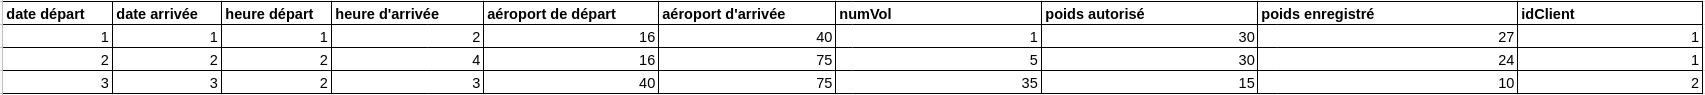
\includegraphics[width=1\textwidth]{img/faitsVentesBillets.png}
  
\end{figure}
\subsection{Dimension date}
\begin{figure}[h]
  \centering
  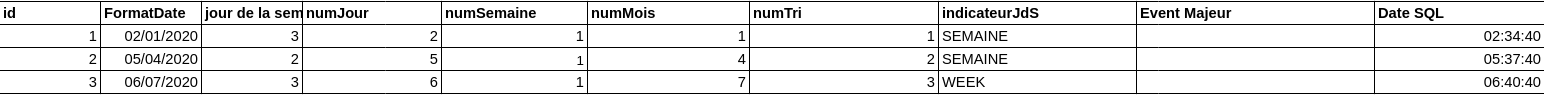
\includegraphics[width=1\textwidth]{img/date.png}
  
\end{figure}

\subsection{Dimension HeureJour}
\begin{figure}[h]
  \centering
  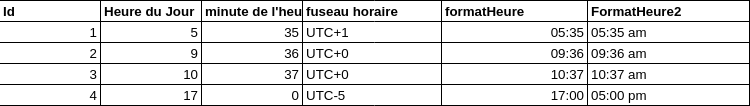
\includegraphics[width=1\textwidth]{img/heureJour.png}
  
\end{figure}



\subsection{Dimension Aéroport}


  
  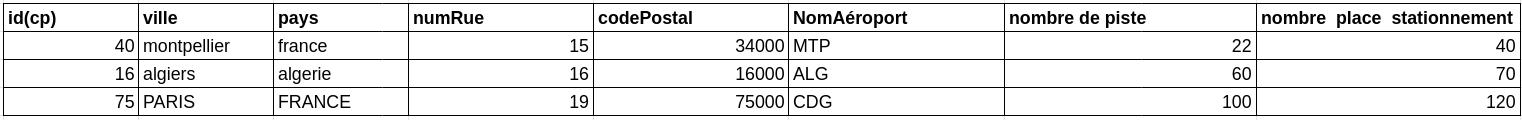
\includegraphics[width=1\textwidth]{img/aeroport.png}
  


\subsection{Dimension Vol}


  
  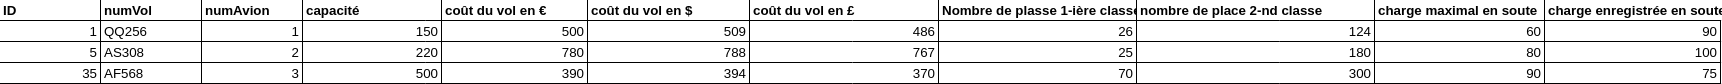
\includegraphics[width=1\textwidth]{img/vol.png}
  




\subsection{Faits flotte d'avions}

  
  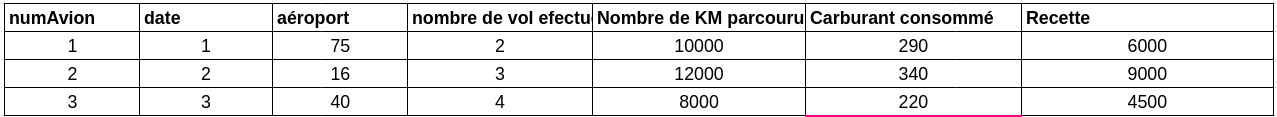
\includegraphics[width=1\textwidth]{img/faitsStockAvions.png}
  


\subsection{Dimension avion}


  
  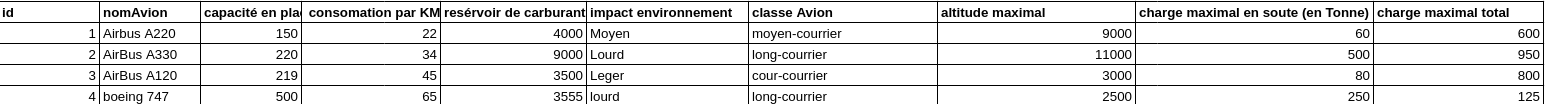
\includegraphics[width=1\textwidth]{img/avion.png}
  




\end{document}
